\documentclass[]{article}
\usepackage[utf8]{inputenc}
\usepackage[T1]{fontenc}
\usepackage{xcolor}
\usepackage{listings}
\usepackage{indentfirst}
\usepackage{hyperref}
\usepackage{graphicx}
\graphicspath{ {.} }
\usepackage{geometry}
\usepackage{multirow}

\geometry{
	a4paper,
	total={170mm,257mm},
	left=20mm,
	top=20mm,
}
\hypersetup{
	colorlinks=true,
	linkcolor=blue,
	filecolor=magenta,      
	urlcolor=cyan,
}

%%
%% Julia definition
%%
\lstdefinelanguage{Julia}%
{morekeywords={abstract,break,case,catch,const,continue,do,else,elseif,%
		end,export,false,for,function,immutable,import,importall,if,in,%
		macro,module,otherwise,quote,return,switch,true,try,type,typealias,%
		using,while},%
	sensitive=true,%
	alsoother={\$},
	morecomment=[l]\#,%
	morecomment=[n]{\#=}{=\#},%
	morestring=[s]{"}{"},%
	morestring=[m]{'}{'},%
}[keywords,comments,strings]%
\lstset{%
	language         = Julia,
	basicstyle       = \ttfamily,
	keywordstyle     = \bfseries\color{blue},
	stringstyle      = \color{magenta},
	commentstyle     = \color{gray},
	showstringspaces = false,
}


%opening
\title{Obliczenia naukowe. Lista nr 3. Sprawozdanie.}
\author{Kacper Szatan, nr 236478}
\date{November 24, 2019}
\begin{document}
\maketitle
\section*{\centering CEL}
Celem listy trzeciej jest zapoznanie się z metodami iteracyjnego wyznaczania miejsc zerowych funkcji na zadanym przedziale i z zadaną dokładnością oraz ich implementacja (zadania 1-3). Zastosowanie poznanych technik do obliczeń (zadania 4-6). Nauka tworzenia modułów w języku Julia.
\section{Zadanie 1}
\subsection{Opis problemu}
W zadaniu pierwszym należało zaimplementować funkcję, która pozwoli na rozwiązanie równania $f(x) = 0$, zadanej funkcji $f$ , z zadaną dokładnością, na zadanym przedziale, metodą bisekcji.
\subsection{Realizacja}
Metoda bisekcji korzysta z własności Darboux dla funkcji ciągłej:\\ Jeżeli $a < b, \: f(a)*f(b)<0$, a obraz funkcji obejmuje cały przedział $[f(a), f(b)]$ to istnieje takie $c \:\epsilon (a, b)$, że $f(c) = 0$. \\
Zatem na początku sprawdzamy czy $f(a)*f(b) < 0$, a właściwie wykonujemy równorzędną operację polegającą na porównaniu znaków: $sign(f(a)) \not= sign(f(b))$. Jeśli nasze porównanie okazuje się nieprawdziwe to znaczy, że funkcja nie ma na tym przedziale zera, które możemy skutecznie wyznaczyć metodą bisekcji. W takim przypadku zwracamy błąd. Jeżeli ten przedział posiada zero to wyznaczamy środek przedziału $[a,b]$ za pomocą przypisania $c = a + (b - a)/2$. Taka forma wyznaczenia środka chroni nas przed wyskoczeniem z przedziału w przypadku ekstremalnych danych. Następnie sprawdzamy, w której z połówek przedziału znajduje się nasze zero (przez porównanie znaku środka i brzegów przedziału). Na koniec iteracji ustalamy połówkę zawierającą zero jako nowy przedział $[a,b]$. Iterując odpowiednią ilość razy otrzymamy w końcu takie $c, \:f(c) = 0$. Jednakże z praktycznego punktu widzenia otrzymanie dokładnie takiego $c$ może być bardzo trudne ze względu na zaokrąglenia arytmetyki, dlatego podajemy parametr \textit{delta}, który określa nam otoczenie $c$. Jeżeli iterując otrzymamy jakieś $c_i \: \epsilon (c-delta, c+delta)$ to kończymy iterowanie i uznajemy za wyniki nasze $c_i$. Metoda bisekcji ma jeszcze jeden warunek stopu. Odpowiada za niego parametr \textit{epsilon}, który jest otoczeniem $0$. Jeżeli dla iteracji $f(c_i) \:\epsilon (-epsilon, epsilon)$ to również należy zakończyć iteracji i wypisać $c_i$ jako wynik.


\section{Zadanie 2}
\subsection{Opis problemu}
W zadaniu drugim należało zaimplementować funkcję, która pozwoli na rozwiązanie równania $f(x) = 0$, zadanej funkcji $f$ , z zadaną dokładnością, metodą Newtona.
\subsection{Realizacja}
Metoda Newtona opiera się na linearyzacji dostarczonej funkcji $f$. Funkcja liniowa, którą zastępujemy orginalną funkcję, powstaje z dwóch pierwszych składników szeregu Taylora. Otrzymujemy równanie rekurencyjne pozwalające obliczać kolejne przybliżenia pierwiastka funkcji $f$. Jest ono postaci $x_{n+1} = x_n - \frac{f(x_n)}{f'(x_n)}$. Algorytm obliczania pierwiastka fukncji metodą Newtona prezentuje się następująco. Na początku sprawdzamy czy pierwsze dostarczone przybliżenie już nie jest tym, którego szukamy. Jeśli tak to je zwracamy. Jeżeli nie to w petli od 1 do podanej maksymalnej liczby iteracji wykonujemy podane kroki:
\begin{itemize}
\item sprawdzamy czy pochodna w $x_0$ jest równa zero. Jeśli jest to przerywamy i wychodzimy z błędem. Jeśli nie to przechodzimy do kolejnego kroku.
\item wyliczamy kolejne przybliżenie ze wzoru $x_{n+1} = x_n - \frac{f(x_n)}{f'(x_n)}$.
\item sprawdzamy czy nowe przybliżenie mieści się w granicach błędu. Jeśli tak to drukujemy wynik. Jeżeli nie to $x_0$ przypisujemy wartość nowego przybliżenia. i powtarzamy pętlę.
\end{itemize}  
Jeżeli opuścimy pętlę bez zwrócenia wyniku to znaczy, że nie udało się w zadanej liczbie iteracji uzyskać pożądanej dokładności.

\section{Zadanie 3}
\subsection{Opis problemu}
W zadaniu trzecim należało zaimplementować funkcję, która pozwoli na rozwiązanie równania $f(x) = 0$, zadanej funkcji $f$ , z zadaną dokładnością, metodą siecznych.
\subsection{Realizacja}
Metoda siecznych powstała przez chęć wyeliminowania kłopotliwego wyliczania pochodnej w metodzie Newtona. W metodzie siecznych wyliczanie pochodnej zostaje przybliżone przez iloraz różnicowy. Otrzymujemy wtedy następujące równanie rekurencyjne na wyliczanie kolejnych przybliżeń pierwiastka funkjci $f$. 
\[x_{n+1} = x_n - \frac{x_n - x_{n - 1}}{f(x_n) - f(x_{n - 1})}f(x_n)\]

Możemy zauważyć, że aby obliczać kolejne przybliżenia potrzebujemy na wejściu dwóch poprzednich przybliżeń. Jednakże w każdym kolejnym kroku korzystamy z wczesniej obliczonych/podanych przybliżeń. Zatem w każdym kroku wyliczamy jeden $x_{n+1}$ wyraz. Następnie tylko raz na krok iteracji korzystamy z podanej funkcji $f$ do wyliczenia wartości $f(x_{n+1})$. 

\section{Wyniki testów}
\begin{table}[h]
	\centering
	\begin{tabular}{||c c c c c||} 
		\hline
		funkcja & metoda & miejsce zerowe & wartość & liczba iteracji \\ [0.5ex] 
		\hline\hline
		\hline
		\multirow{3}{*}{$x^5 - 2x^4 - 24x^3 $} 
		&bisekcja& 5.999977111816406 & -0.049437797631981084 & 17  \\
		&Newton& 6.000000000391925 & 8.465567589155398e-7 & 9 \\
		&sieczne& 6.000000010294027 & 2.2235098185774405e-5 & 12 \\
		\hline
		\multirow{3}{*}{$x^2-9$} 
		&bisekcja& 3.0000228881835938 & 0.00013732962543144822 & 17 \\
		&Newton& 3.000000001396984 & 8.381903171539307e-9 & 5 \\
		&sieczne& 3.0000001572864043 & 9.43718450940878e-7 & 6 \\
		\hline
		\multirow{3}{*}{$sin(x)*3x^2$} 
		&bisekcja & 0.03125 & 9.1537833941385e-5 & 5 \\
		&Newton & 3.141592657586969 & -1.1835163193721654e-7 & 4\\
		&sieczne& 3.1415923324542794 & 9.508439498873873e-6 & 3 \\
		\hline
		\multirow{3}{*}{$cos(3 * x^6) + 17 * x^(-3) - 35*x^2$} 
		&bisekcja& 0.8674125671386719 & 0.0024714700019892177 & 16 \\
		&Newton& 0.8674278904924629 & 3.0962019469171764e-5 & 7 \\
		&sieczne& 0.8674280834971032 & 2.2311705905053714e-7 & 8 \\
		\hline
	\end{tabular}
	\caption{Zaprezentowane wyniki otrzymano przy $\delta\:,\epsilon = 10^{-4}$. Umiejscowienie miejsc zerowych kontrolowano za pomocą Wolfram Alpha.}
\end{table}

\section{Wnioski z zadań 1, 2 i 3}
Metoda bisekcji jest zdecydowanie najwolniejsza z tych trzech. Jest ona zbieżna liniowo. To znaczy, że dla ciągu $\{x_n\}$, który zbiega do $r$ istnieje stała $C < 1$ oraz $\alpha = 1$ takie że: \[(1) \: \: \:|x_{n+1} - r| \leq C|x_n - r|^\alpha\] Jednakże metoda bisekcji ma tą zaletę, że jest globalnie zbieżna. To znaczy, że dla każdego $a$ i $b$ takiego, że $f(a)*f(b) < 0$ metoda ta znajdzie miejsca zerowe. Dlatego zaleca się stosowanie jej hybrydowa z innymi metodami, które są zbieżne lokalnie (Newton, siecznych). 
\\
Metoda Newtona jest szybka, ponieważ jest zbieżna kwadratowo czyli $\alpha = 2$ w nierówności $(1)$. Niestey jest zbieżna tylko lokalnie i wymaga wyliczenia i dzielenia przez pochodną funkcji, którą chcemy przybliżać. Co może być problemem gdy pochodna jest bliska zeru.
\\
Metoda siecznych eliminuje problem z wyliczaniem pochodnej w metodzie newtona, ale wciąż jest zbieżna jedynie lokalnie, a nie jest już zbieżna kwadratowo. To znaczy w jej przypadku w równaniu $(1)$ $\alpha \approx 1.618$. Zatem jest nieco wolniejsza niż metoda Newtona.
\\\\
Pseudokody dla metod opracowanych w zadaniach 1-3:
\hrule
\begin{lstlisting}
mbisekcji(f, a, b, delta, epsilon)
leftV = f(a)
rightV = f(b)
it = 0
# sprawdzenie czy 'f' przechodzi przez zero 0. 
if sign(leftV) == sign(rightV)
 return -1, -1, it, 1 # ERROR
end 
range = b - a 
while range > epsilon # (tu mozna ograniczyc tez maksymalna liczbe iteracji)
 it = it + 1
 range = range / 2 
 r = a + range   
 v = f(r)    
 if abs(range) < delta OR abs(v) < epsilon 
  return r, v, it, 0 # ANSWER  
 end
 if sign(leftV) != sign(v) #leftV = f(a) i rightV = f(b)
  b = r
  rightV = v
 else
  a = r
  leftV = v
 end
return a, f(a), it, 1 # ERROR/ANSWER  Jesli wynik nie zostal wyliczony,
# a nie mozna juz zmniejszac przedzialu.
end
\end{lstlisting}
\textit{Listing 1: Metoda bisekcji.}
\\\\\hrule
\begin{lstlisting}
mstycznych(f,pf,x0, delta, epsilon, maxit)
v = f(x0)
r = x0
it = 0
if abs(v) < epsilon # xO jest dobra aproksymacja juz na poczatku
 return r, v, it, 0
end
for it = 1 : maxit
 if (abs(pf(x0)) < epsilon) # sprawdzenie czy pochodna nie jest bliska zero
  return (r, v, it, 2)
 end 
 r = x0 - (v / pf(x0))  
 v = f(r)           
 if(abs(r - x0) < delta || abs(v) < epsilon) 
  return r, v, it, 0
 end
 x0 = r              
end
return r, v, it, 1  # nie znaleziono wyniku w zadanej liczbie iteracji
\end{lstlisting}
\textit{Listing 2: Metoda Newtona (stycznych).}
\newpage
\hrule
\begin{lstlisting}
function msiecznych(f, x0, x1, delta, epsilon, maxit)
x0r = x0
x1r = x1
x0v = f(x0)         
x1v = f(x1)  
it = maxit    
for it = 1 : maxit	# liczba iteracji = maxit
 if (abs(x0v) > abs(x1v))    # ustawiamy tak by f(x0) < f(x1) 
  x0r, x1r = x1r, x0r 
  x0v, x1v = x1v, x0v 
 end 
 #x_0 = x_n | x_1 = x_n-1
 diff = (x0r - x1r)/(x0v - x1v)  # iloraz roznicowy
 x1r = x0r               #  x_n to nowe x_n-1
 x1v = x0v               #  f(x_n) to nowe f(x_n-1)
 x0r = x0r - (x0v * diff)         # wyliczamy nowe przyblizenie.
 #Przeciecie siecznej z osia OX 
 x0v = f(x0r)                 # wartosc nowego przyblizenia
 if (abs(x1r - x0r) < delta || abs(x0v) < epsilon)     # warunki konca
  return x0r, x0v, it, 0
 end
end
return x0r, x0v, it, 1   # nie osiagnieto wymaganej dokladnosci '1'
end

\end{lstlisting}
\textit{Listing 3: Metoda siecznych.}
\section{Zadanie 4}
\subsection{Opis problemu}
Z użyciem wcześniej zaimplementowanych metod należało wyliczyć pierwiastek równania $sin\: x - (\frac{1}{2}x)^2 = 0$. Eksperymenty przeprowadzono w dokładności $\delta = \frac{1}{2}10^{-5}, \:\:\: \epsilon = \frac{1}{2}10^{-5}$. Lista eksperymentów:
\begin{itemize}
	\item[1.] bisekcja na przedziale $[1.5, 2]$
	\item[2.] Newton z przybliżeniem początkowym $x_0 = 1.5$ 
	\item[3.] sieczne z przybliżeniami początkowymi $x_0 = 1, \:\: x_1 = 2$ 
\end{itemize}
\subsection{Realizacja}
Zaimplementowano funkcje $f(x) = sin\: x - (\frac{1}{2}x)^2$ oraz jej pochodną $df(x) = cos\: x - (\frac{1}{2}x)$. Obliczenie postaci pochodnej jest wymagane przy zastosowaniu metody Newtona. Maksymalną liczbę iteracji ustalono na 25. Następnie skorzystano z wcześniej zaimplementowanych metod.
\subsection{Wyniki}
\begin{table}[h]
	\centering
	\begin{tabular}{||c c c c||} 
		\hline
		metoda & miejsce zerowe & wartość & liczba iteracji \\ [0.5ex] 
		\hline\hline
		bisekcja & 1.9337539672851562 & -2.7027680138402843e-7 & 16 \\
		Newton & 1.933753779789742 & -2.2423316314856834e-8 & 4 \\
		sieczne & 1.933753644474301 & 1.564525129449379e-7& 4 \\
		\hline
	\end{tabular}
	\caption{Zaprezentowane wyniki otrzymano przy $\delta\:,\epsilon = \frac{1}{2}10^{-5}$.}
\end{table}
\subsection{Wnioski}
Przprowadzony eksperyment pozwala nam na zobaczyć zależności pomiędzy metodami. Od razu widać, że metoda bisekcji jest najwolniejsza z powodu swojej liniowej zbieżności. Co było już omawiane w punkcie 5. Aby odnaleźć miejsce zerowe w zadanej dokładności metoda bisekcji potrzebowała aż 16 kroków, gdy metody Newtona i siecznych zaledwie 4. Metoda Newtona pozwoliła nam otrzymać najdokładniejszy wynik (najbliżej zera). Jednakże wszystkie trzy metody zwróciły wynik mieszczący się w zadanej dokładności. Aby lepiej zbadać różnice w prędkości biegania metody Newtona oraz siecznych przeprowadzono jeszcze jeden test. Polegał on na zmianie początkowych przybliżeń podawanych do metody siecznych oraz metody stycznych. Dla Newtona podano początkowe przybliżenie jako $x_0 = 150.0$, a w metodzie siecznych $x_0 = 100.0, \:\:x_1 = 200.0$. Dla tych parametrów metoda Newtona zakończyła eksperyment po 8 krokach a metoda stycznych po 12. Co dobrze ilustruje różnice w prędkości zbieżności. Newton - zbieżność kwadratowa $\alpha = 2$. Metoda siecznych - zbieżność nadliniowa $\alpha \approx 1.6$.   
\section{Zadanie 5}
\subsection{Opis problemu}
W zadaniu 5 należało metodą bisekcji wyznaczyć wartość zmiennej $x$, dla której wykresy funkcji $y = 3x$ i $y = e^x$ przecinają się. Eksperyment należało przeprowadzić z dokładnością $\delta = 10^{-4}$, $\epsilon = 10^{-4}$.
\subsection{Realizacja}
Łatwo zauważamy, że problem redukuje się do znalezienia pierwiastków równania $e^x - 3x = 0$. Dlatego definiujemy anonimową funkcję $f(x) = e^x - 3x$. Pozwala nam to na skorzystanie z wcześniej zaimplementowanej metody bisekcji. Aby wyznaczyć przedziały skorzystano z programu Wolfram Alpha do wizualizacji dwóch zadanych funkcji. 
\\
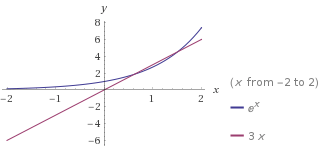
\includegraphics{plot}
\\ 
Pobierzna analiza wykresu pozwoli nam  na wyznaczenie dwóch przedziałów w których znajdują się miejsca zerowe utworzonej przez nas funkcji anonimowej $f$. Zaproponowane przedziały to $(0, 1)$ oraz $(1, 2)$.
\subsection{Wyniki}
\begin{table}[h]
	\centering
	\begin{tabular}{||c c c c||} 
		\hline
		przecięcie & miejsce zerowe & wartość & liczba iteracji \\ [0.5ex] 
		\hline\hline
		$x_1 \epsilon [0, 1]$ & 0.619140625 & -9.066320343276146e-5 & 9 \\
		
		$x_2 \epsilon [1, 2]$ & 1.5120849609375 & -7.618578602741621e-5 & 13 \\
		\hline
	\end{tabular}
	\caption{Zaprezentowane wyniki otrzymano przy $\delta\:,\epsilon = 10^{-4}$.}
\end{table}
\subsection{Wnioski}
Po odpowiednim przeformułowaniu zadania jesteśmy w stanie z powodzeniem szukać miejsc przecięć wykresów zadanych funkcji korzystając z metod iteracyjnych. Głównym problemem jest lokalizacja właściwych przedziałów początkowych. Możemy skorzystać tutaj z pomocy wykresu podanych funkcji lub oparzeć się o naszą znajomość/intuicję przebiegu funkcji $f$. 
\section{Zadanie 6}
\subsection{Opis problemu}
W zadaniu 6 należało znaleźć miejsce zerowe funkcji $f_1(x) = e^{1-x}-1$ oraz $f_2(x) = xe^{-x}$ za pomocą metod bisekcji, Newtona i siecznych. Wymagane dokładności obliczeń: $\delta = 10^{-5}, \:\: \epsilon = 10^{-5}$. Należało dobrać odpowiednio przedział i przybliżenia początkowe.
\subsection{Realizacja}
Funkcje $f_1$ i $f_2$ zostały zaimplementowane wraz z ich pochodnymi. Następnie aby wzynaczyć właściwe przedziały dla metody bisekcji ora przyblienia początkowe dla metody siecznych oraz stycznych, przeanalizowano wykresy funkcji. Wykresy zwizualizowano za pomocą porgamu Wolfram Alpha. Poniżej zamieszczono interesujący nas kawałek wykresu w którym znajdują się miejsca zerowe obu tych funkcji.  
\\
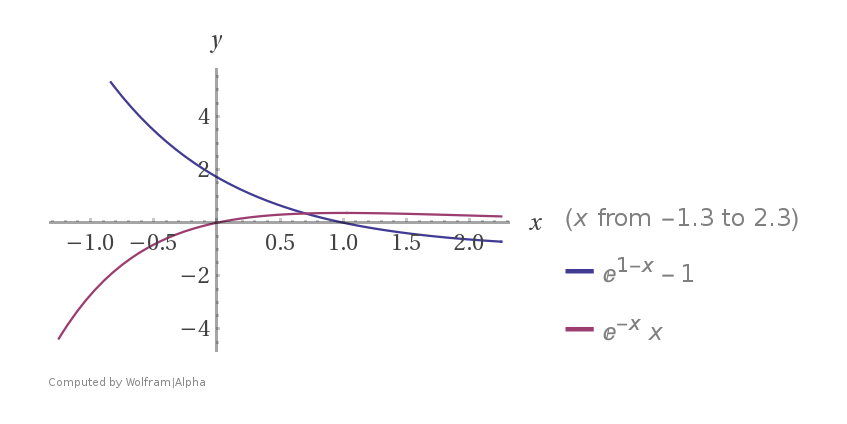
\includegraphics[scale =0.5]{plot2}
\subsection{Wyniki}
\begin{table}[h]
	\centering
	\begin{tabular}{||c c c c c c c||} 
		\hline
		Funkcja & Przedział & Metoda & Miejsce Zerowe & Wartość & Liczba Iteracji & Błąd \\ [0.5ex] 
		\hline\hline
		\multirow{3}{*}{$f_1(x) = e^{1-x}-1$} &
		$[0, 2.5]$ & bisekcja & 1.0000038146972656 & -3.814689989667386e-6 & 17 & 0\\
		&$0$ & Newton & 0.9999984358892101 & 1.5641120130194253e-6 & 4 & 0\\
		&$-0.5,\: 0 $ & sieczne & 0.9999997759095745 & 2.2409045064009092e-7&
		 6 & 0\\
		\multirow{3}{*}{$f_2(x) = xe^{-x}$} &
		$[-1, 1.5]$ & bisekcja & 3.814697265625e-6 & 3.814682713737527e-6 & 17 & 0\\
		&-1 & Newton & -3.0642493416461764e-7 & -3.0642502806087233e-7 & 5 &  0\\
		& -1.5, -1 & sieczne & -1.724632957993133e-6 & -1.7246359323545378e-6 & 7 & 0\\
		\hline
		\multirow{3}{*}{$f_1(x) = e^{1-x}-1$} &
		
		
		$[0, 5.0]$ & bisekcja & 1.0000038146972656 & -3.814689989667386e-6 & 18 & 0\\
		&$5.5$ & Newton & 0.9999998543788339 & 1.4562117667260566e-7 & 89 & 0\\
		&$5,\: 7.5 $ & sieczne & 5.0 & -0.9816843611112658 & 2 & 0\\
		\multirow{3}{*}{$f_2(x) = xe^{-x}$} &
		$[-1, 100]$ & bisekcja & 49.5 &  1.574085595597886e-20 & 1 & 0\\
		& 1 & Newton & 1.0 & 0.36787944117144233 & 1 &  2\\
		& 1.5, 1 & sieczne & 14.633260759544537 & 6.459467411373784e-6 & 12 & 0\\
		\hline
		\multirow{3}{*}{$f_2(x) = xe^{-x}$} &
		$[-10, 1000]$ & bisekcja & 495.0 &  5.234035414371182e-213 & 1 & 0\\
		& 10 & Newton & 14.380524159896261 & 8.173205649825554e-6 & 4 &  0\\
		& 10.5, 10 & sieczne & 14.36657792367032 &8.279951953887678e-6 & 5 & 0\\
		\hline
	\end{tabular}
	\caption{Zaprezentowane wyniki otrzymano przy $\delta\:,\epsilon = 10^{-5}$.}
\end{table}
\subsection{Wnioski}
Aby w pełni zrozumieć problem należy poddać głębszej analizie podane w zadaniu funkcje. Oprócz wyznaczenia przedziałów w których znajdują się miejsca zerowe przydatną informacją jest również to że funkcja $\lim_{x\to\infty} f_1(x) = -1$ oraz $\lim_{x\to\infty} f_2(x) = 0$. Te informacje pozwalają nam na właściwie zinterpretowanie niektórych wyników, które mogą wydawać się absurdalne. W pierwszym bloku w tabeli czwartej mamy przedziały oraz przybliżenia początkowe dobrane właściwie. W konsekwencji pozwala nam to na właściwe wyliczenie miejsc zerwoych z zadaną dokładnością. W drugim bloku tabeli 4 ilustrujemy co się stanie gdy przybliżenia początkowe dla $f_1$ będą większe od 1. Metoda bisekcji jedynie zwiększa liczbę iteracji, ale wciąż zwraca prawidłowy i pożądany wynik w rozsądnym czasie (liczbie iteracji). W metodzie Newtona drastycznie zaczyna wzrastać liczba iteracji potrzebna do obliczenia miejsca zerowego. Jest to związane z $\lim_{x\to\infty} f_1(x) = -1$. Dla $x>1$ funkcja $f_1$ zaczyna coraz bardziej przypominać stałą. Więc pochodna tej funkcji coraz bardziej zbliża się do zera. Podczas linearyzacji prawie 'stałego' odcinka wykresu kolejne styczne prawie pokrywają się z wykresem faktycznym co prowadzi do bardzo powolnego wyznaczania miejsca zerowego, gdyż kolejne przybliżenia są bardzo blisko siebie. Gdy weżniemey odpowiednio duży $x$ jako przybliżenie początkowe może się zdażyć, że pochodna będzie na tyle blisko zera, że nie możliwe okaze się zastosowanie metody Newtona. Metoda siecznych choć nie zwraca błędu nie doprowadza nas do właściwego wyniku. Doszło do sytuacji w której odległość między kolejnymi przybliżeniami jest mniejsza niż zadeklarowana $\delta = 10 ^{-5}$. Co jest jednym z warunków końca metody siecznych. Niestety nie otrzymujemy wtedy wiarygodnego wyniku.
\\Natomiast gdy zmodyfikujemy przedziały w funkcji $f_2$ efekt jest następujący. Bisekcja niestety zwraca nam wynik nieprawdziwy. Ma to związek z samą funkcją, której granica w nieskończoności jest równa zero. Dlatego gdy wybierzemy odpowiednio duże $x$ wartość funkcji jest bliska zeru i iteracja zostaje przerwana bo zostaje spełniony warunek $f(x) < \epsilon$. Niestety nie znajdujemy się nawet w okolicy miejsca zerowego. Gdy zastosujemy metodę Newtona z przybliżeniem początkowym $x_0 = 1$ to pochodna $f_2$ przyjmuje wtedy zero, zatem niemożliwe jest zastosowanie tej metody. Informuje nas o tym komunikat błędu z wyjściem 2. Gdy zaczniemy wybierać przybliżenia początkowe wieksze niż 1 znów wpadniemy w pułapkę (granica w nieskończoności $f_2 = 0$ ). Wartości wtedy są bardzo bliskie zera, ale nie znajdujemy się w pobliżu miejsca zerowego. Zostanie nam zwórcone wtedy pierwszze przybliżenie dla którego wartośći jest mniejsza niż zadeklarowany epsilon. Zwiększając dokładność (to znaczy zmniejszajac wartość epsilona), będziemy jedynie oddalać się od faktycznego miejsca zerowego tej funkcji. Metoda siecznych reaguje podobnie. Z wyjątkiem $x_0 = 0$, gdzie rozbiega się w strone granicy, zamiast (jak byśmy chcieli) zbiegać do miejsca zerowego.
%Sprawdzić co stanie, gdy w metodzie Newtona dla f1 wybierzemy x0∈(1,∞] a dla f2 wybie-rzemy x0>1, czy mogę wybrać x0= 1 dla f2
\end{document}